\documentclass{seminar}

% Use latex filename for dvi output and pdflatex file for pdf output.

\usepackage[dvips]{graphicx}

% \usepackage[pdftex]{graphicx} does not seem to be needed.

\DeclareGraphicsExtensions{.eps,.ps,.pdf,.jpg}

\usepackage{alltt} % 
\usepackage{fancybox} % For making Oval borders.
\usepackage{amssymb}  % For, for example, \mathbb, \big, and \mapsto
\usepackage{url} % For email addresses, hypertext links, ...
\usepackage{color} % For color.
\usepackage{hyperref} % For hyper reference but *essential* for seminar.
\usepackage{multicol}
\definecolor{green}{rgb}{0,0.8,0}
% Options for hyperref.

\hypersetup{pdfpagemode=none,pdfstartview=FitH} % For the initial view.
\hypersetup{colorlinks=true}
\hypersetup{hypertexnames=false} % Eliminates message: pdfTeX warning (ext4)
\hypersetup{urlcolor=red}

% Basic definitions.

\renewcommand{\printlandscape}{\special{landscape}}    % Works with dvips.
\newcommand{\R}{\mbox{${\mathbb R}$}}
\newcommand{\C}{\mbox{${\mathbb C}$}}
\newcommand{\grad}{\nabla}
\setlength{\jot}{0.0pt}
\newcommand{\half}{{\textstyle{\frac{1}{2}}}}
\newcommand{\third}{{\textstyle{\frac{1}{3}}}}
\newcommand{\codes}[1]{{\textsf{\footnotesize #1}}}

% Calligraphic letter abbreviations.

\newcommand{\cA} {\mbox{$\cal A$}}
\newcommand{\cP} {\mbox{$\cal P$}}
\newcommand{\cS} {\mbox{$\cal S$}}
\newcommand{\cT} {\mbox{$\cal T$}}

% Color symbols.

\newcommand{\redball}{\textcolor{red}{$\bullet$}}
\newcommand{\reddash}{\textcolor{red}{$--$}}
\newcommand{\reddiamond}{\textcolor{red}{$\diamond$}}
\newcommand{\blackdiamond}{\textcolor{black}{$\diamond$}}
\newcommand{\redcircle}{\textcolor{red}{$\circ$}}
\newcommand{\redstar}{\textcolor{red}{$\star$}}
\newcommand{\redrightarrow}{\textcolor{red}{$\Rightarrow$}}

\newcommand{\redstripe}{\textcolor{red}{\hrule height 2.0pt\hfil}
             \vspace{-1.8pt}
             \textcolor{red}{\hrule height 1.0pt\hfil}
}

\newcommand{\heading}[1]{%
   \centerline{\textcolor{blue}{\textbf{#1}}}%
    \redstripe%
    \bigskip
}

% Script letters.

\newcommand{\cD} {\mbox{$\cal D$}}

%\newpagestyle{MH}{}
%{
%\ifpdf
%\hfil 
\includegraphics[height=0.35in]{../images/lans_logo}
%\else
%\fi
%}

%\newpagestyle{MH}{}
%{\hfil http://www.mcs.anl.gov/tao  \hfil}
%{\hfil \thepage \hfil}


%\pagestyle{MH}
\pagestyle{empty}

\slideframe{Oval}
\slideframe{none}

% \twoup

\begin{document}

\begin{slide}

\begin{center}
{\bf
%\textcolor[named]{mycolor}{Just testing colors}
Workshop on the ACTS Toolkit \\
September 4--7, 2002 \\
National Energy Research Scientific Computing Center
}
\end{center}

\redstripe

\begin{center}
{\bf
\textcolor{blue}{TAO -- Toolkit for Advanced Optimization}
}

\redstripe

\medskip

\centerline{\bf Steve Benson, Lois Curfman McInnes} 
\centerline{\bf Jorge J. Mor\'e, and Jason Sarich}

\end{center}

% \medskip

\parbox[b]{3in}{\bf http://www.mcs.anl.gov/tao \bigskip \\
\small  Mathematics and Computer Science Division \\ 
Argonne National Laboratory} 
\includegraphics[scale=0.5]{../images//argonne}

\end{slide}


\begin{slide}

\heading{What is Nonlinearly Constrained Optimization?}

\[
\min \left \{ f(x): x_l \le x \le x_u , \ c_l \le c(x) \le c_u \right \}
\]

\medskip

\begin{list}{\reddiamond}
{
% \setlength{\itemsep}{0pt}
}
\item
Unconstrained optimization
\[
\min \left \{  f(x) : x \in \R^n \right \}
\]
\item
Bound-constrained optimization
\[
\min \left \{  f(x) : x_l \le x \le x_u \right \}
\]
\item
Linear and quadratic programming
\[
\min \left \{ \half x^T Q x + c^T x : x_l \le x \le x_u , 
\ c_l \le Ax \le c_u \right \}
\]
\end{list}

\vfill

\end{slide}


\begin{slide}

\heading{What is Nonlinearly Constrained Optimization?}

\[
\min \left \{ f(x): x_l \le x \le x_u , \ c_l \le c(x) \le c_u \right \}
\]

\medskip

\begin{list}{\reddiamond}
{
% \setlength{\itemsep}{0pt}
}
\item
Systems of nonlinear equations
\[
\min \left \{ \half \| r(x) \|^2 : x_l \le x \le x_u \right \} , \qquad
r : \R^n \mapsto \R^n
\]
\item
Nonlinear least squares
\[
\min \left \{ \half \| r(x) \|^2 : x_l \le x \le x_u \right \} , \qquad
r : \R^n \mapsto \R^m, \quad m \ge n
\]
\end{list}

\vfill

\end{slide}



\begin{slide}

\heading{The Ginzburg-Landau Model for Superconductivity}

Minimize the Gibbs free energy for a homogeneous superconductor with a vector
potential perpendicular to the superconductor.

{\small
\[
\int _ {\cD} \bigl \{ - | v (x) |^2 + \half | v (x) |^4  + 
\left \| \left [ \nabla - i A(x) \right ] v (x) \right \| ^2  +  \\
\kappa^2 \left \| ( \grad \times A ) (x) \right \| ^2 \bigr \} dx
\]
}

\medskip

\begin{center}
$ v : \R^2 \to \C$ is the order parameter

$A : \R^2 \to \R^2 $ is the vector potential
\end{center}

\vfill

\end{slide}

\begin{slide}

\heading{The Ginzburg-Landau Model for Superconductivity}

Unconstrained problem. Non-convex function. Hessian is singular.
Unique minimizer, but there is a saddle point.

\centerline {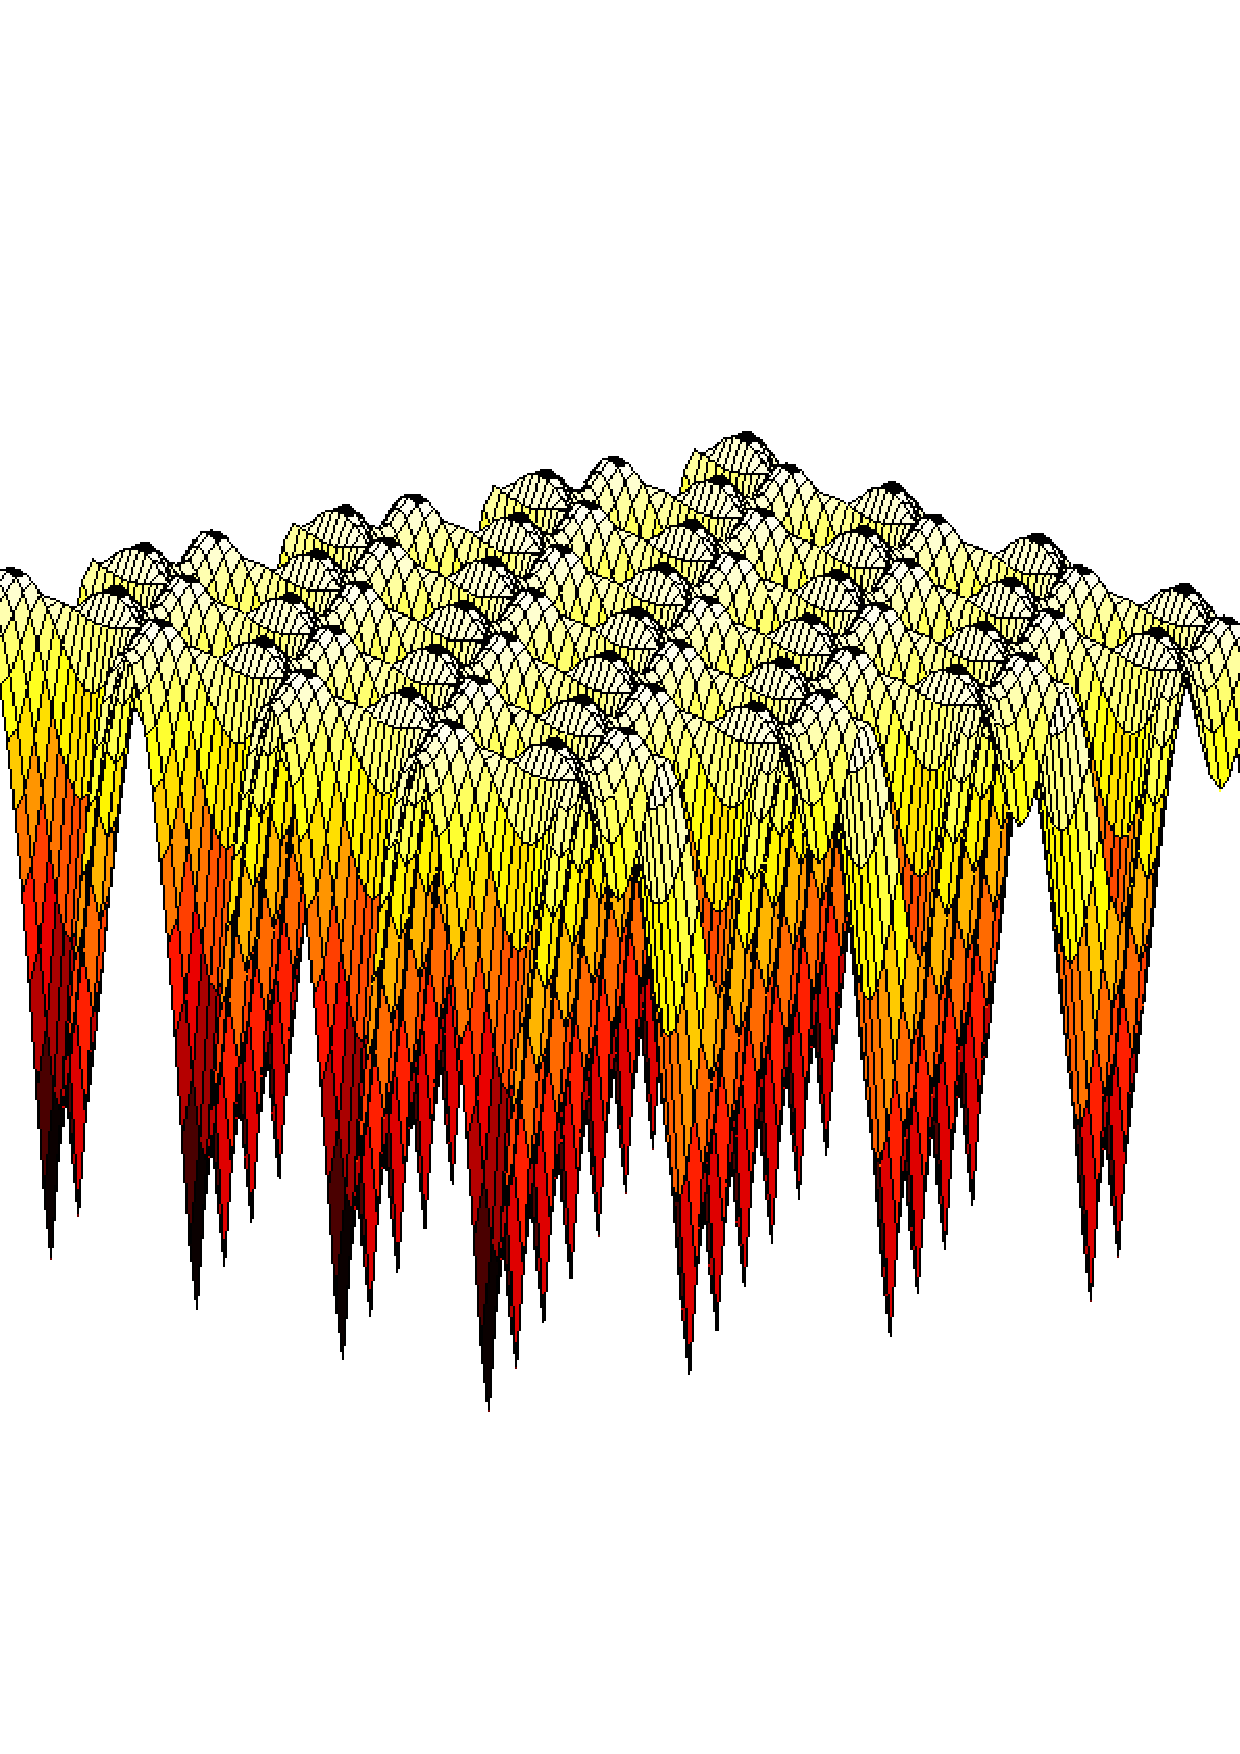
\includegraphics[height=1.9in]{../images/gl2}}

\end{slide}

\begin{slide}

\heading{Pressure Distribution in a Journal Bearing}

Determine the pressure distribution in a thin film of lubricant
between two circular cylinders

\[
\int_{\cD} \Bigl \{ \half w_q (x) \| \grad v(x) \|^2 - w_l(x) v(x) \Bigr \} \; dx
\]

\[
w_q ( \xi_1 , \xi_2 ) = \left ( 1 + \varepsilon \cos(\xi_1) \right ) ^ 2
\]
\[
w_l ( \xi_1 , \xi_2 ) =  \varepsilon \sin (\xi_1)
\]

\medskip

\begin{center}
$ v \ge 0 $ on the domain $ \cD = ( 0 , 2 \pi ) \times ( 0 , 2 b ) $.
\end{center}

\vfill

\end{slide}

\begin{slide}

\heading{Pressure Distribution in a Journal Bearing}

Bound constrained problem. 
Number of active constraints depends on the eccentricity $ \varepsilon $.
Badly scaled Hessian matrix.
%
\centerline {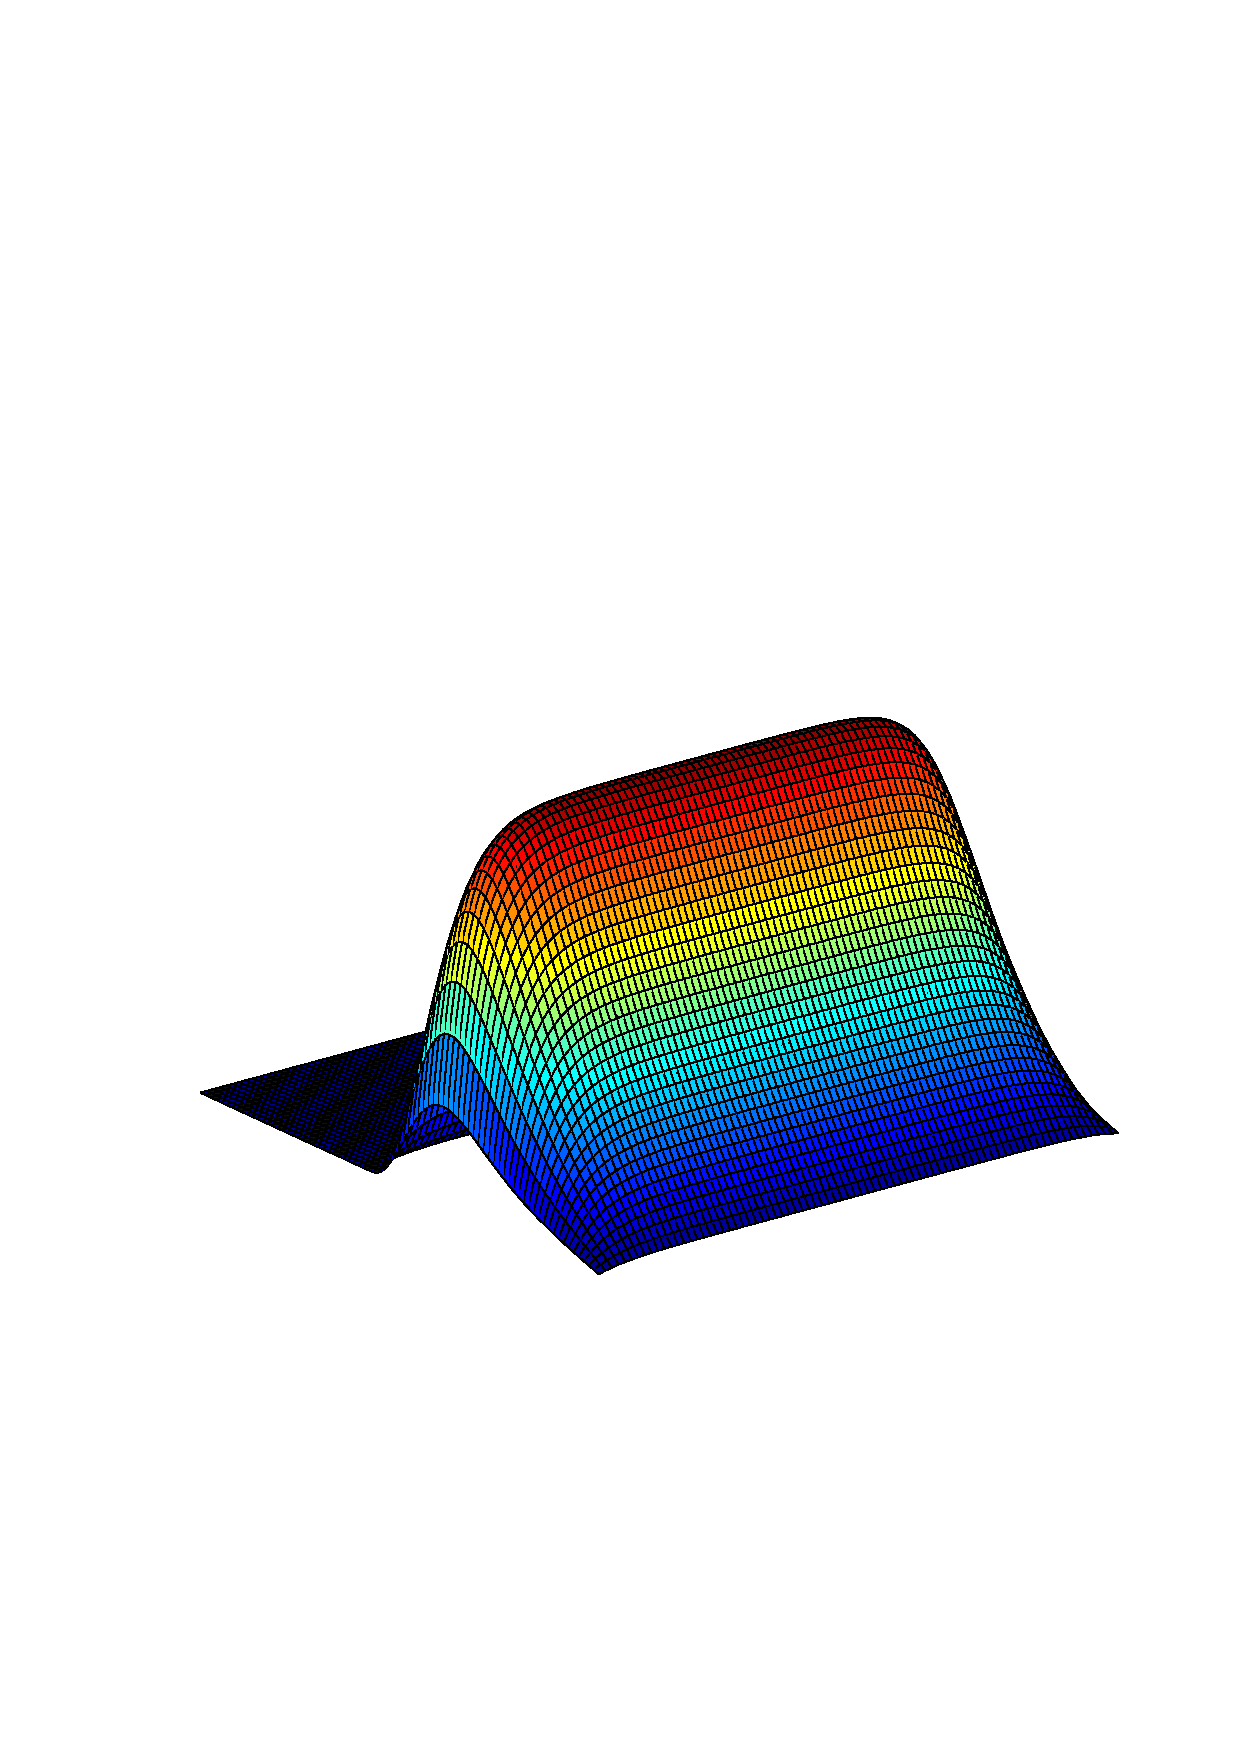
\includegraphics[height=2.0in]{../images/pjb}}

\end{slide}


\begin{slide}

\heading{Minimal Surface with Obstacles}

Determine the surface of minimal area and given boundary data
that lies above an obstacle.

\[
\min \left \{ f(v) : v \in K \right \}
\]

\[
f(v) = \int_{\cD} \sqrt{ 1 + \| \grad v(x) \|^2 } \; dx
\]

\[
K = \left \{ v \in H^1 : v(x) = v_D (x) , \ x \in \partial D, \ 
                v(x) \ge v_L (x) ,\  x \in \cD \right \}
\]

\vfill

\end{slide}

\begin{slide}

\heading{Minimal Surface with Obstacles}

Bound constrained problem. 
Number of active constraints depends on the height of the
obstacle. All multipliers are zero. 
%
\centerline {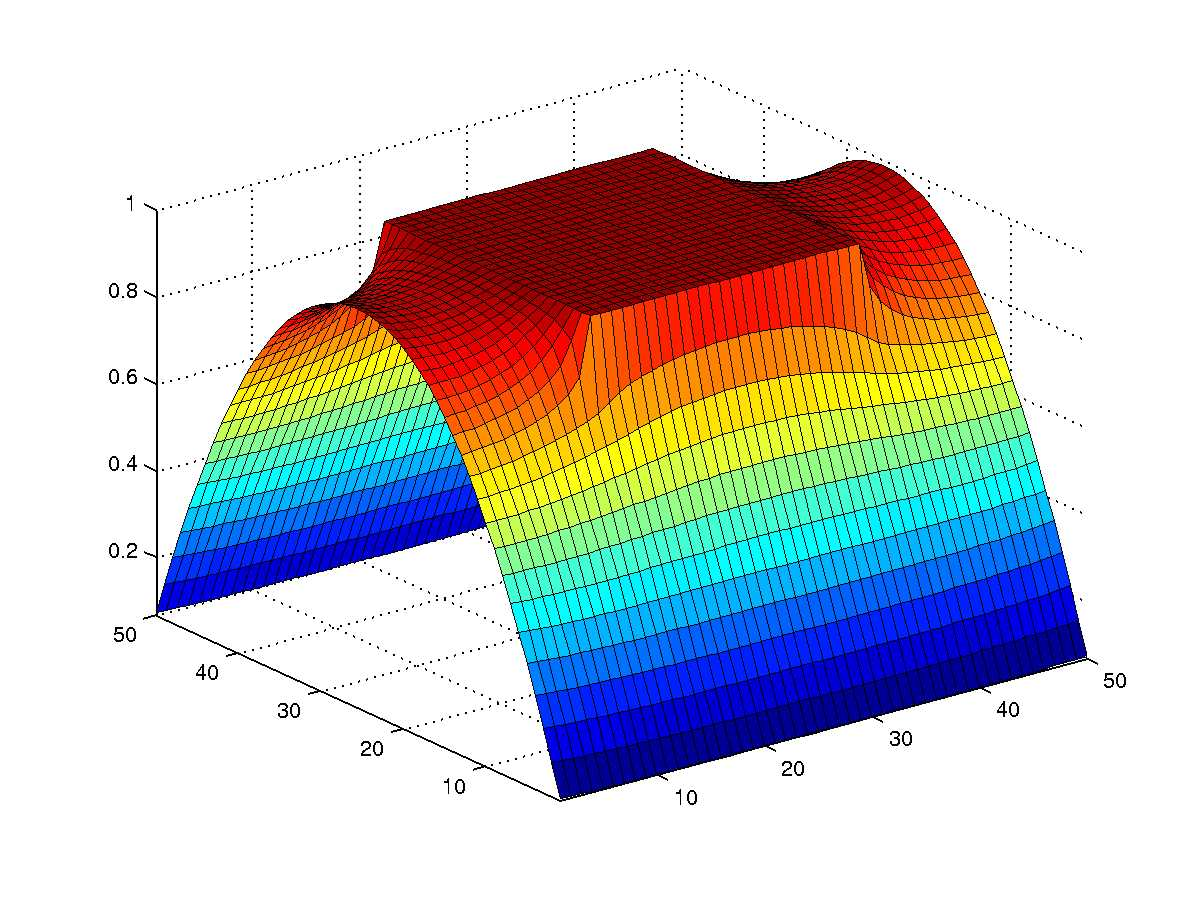
\includegraphics[height=2.0in]{../images/mso}}

\end{slide}

\begin{slide}

\heading{Isomerization of $ \alpha $-pinene}

Determine the reaction coefficients
in the thermal isometrization of $\alpha$-pinene from measurements by minimizing
\[
\sum _ {j=1}^8 \| y ( \tau_j ; \theta ) - z_j \| ^ 2 ,
\]
where $z_j$ are the measurements and
\begin{eqnarray*}
y_1'  & = & -(\theta_1 + \theta_2) y_1 \\
y_2'  & = & \theta_1 y_1 \\
y_3'  & = & \theta_2 y_1 - (\theta_3 + \theta_4 )y_3 + \theta_5 y_5 \\
y_4'  & = & \theta_3 y_3 \\
y_5'  & = & \theta_4 y_3 - \theta_5 y_5 \nonumber
\end{eqnarray*}

\vfill

\end{slide}

\begin{slide}

\heading{Isomerization of $\alpha$-pinene}

Only equality constraints. Typical parameter estimation problem. 

\bigskip

\centerline {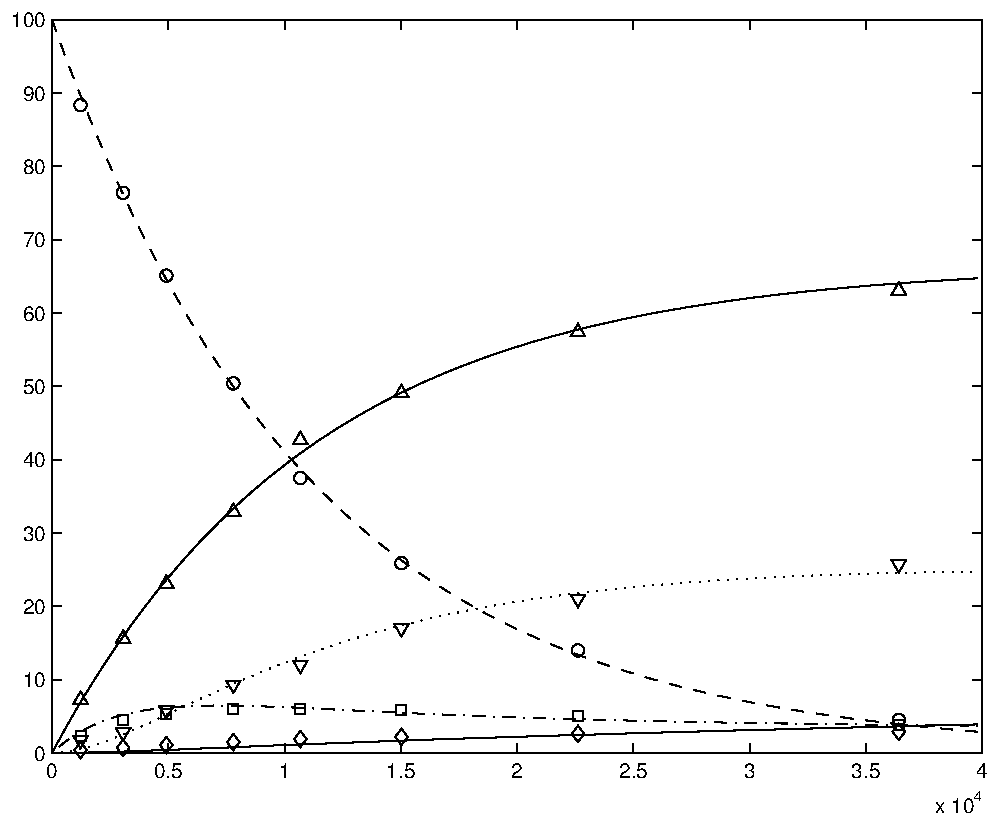
\includegraphics[height=1.8in]{../images/pinene}}

\vfill

\end{slide}

\begin{slide}

\heading{Optimization Toolkits}

State-of-the-art in optimization software:

\begin{list}{\reddiamond}{}
\item
Scattered support for parallel computations
\item
Little reuse of linear algebra software
\item
Minimal use of automatic differentiation software
\item
Rigid assumptions about data representations
\item
Nonlinear optimization problems with more than $ 10, 000 $
variables are considered large.
\end{list}

\vfill

\end{slide}

\begin{slide}

\heading{TAO}

The process of nature by which all things change
and which is to be followed for a life of harmony.

\bigskip

\begin{center}
\textcolor{red}{The Right Way}
\end{center}

\bigskip

Toolkit for Advanced Optimization

\begin{list}{\reddiamond}{}
\item
Object-oriented techniques
\item
Component-based interactions
\item
Leverage of existing parallel computing infrastructure
\item
Reuse of external toolkits
\end{list}

\vfill

\end{slide}

\begin{slide}

\heading{TAO Goals}

\begin{list}{\reddiamond}{}
\item
High performance
\item
Scalable parallelism
\item
Portability
\item
An interface independent of architecture
\end{list}

\vfill

\end{slide}


\begin{slide}

\heading{TAO Algorithms (partial list)}

\begin{list}{\reddiamond}
{ \setlength{\itemsep}{0pt}}
\item
Unconstrained optimization 
\begin{list}{\reddash}{}
\item
Conjugate gradient algorithms PR, FR, PR+
\item
Newton line search and trust region
\end{list}
\item
Bound-constrained optimization
\begin{list}{\reddash}{}
\item
Limited-memory variable-metric algorithm
\item
Trust region Newton method
% \item
% Gradient projection/conjugate gradient algorithm
\end{list}

\item Complementarity
\begin{list}{\reddash}{}
\item Semismooth methods
\end{list}
%\item
%Linearly constrained optimization
%\begin{list}{\reddash}{}
%\item
%Interior-point quadratic programming  method (alpha)
%\end{list}
\end{list}

\vfill

\end{slide}

\begin{slide}

\heading{TAO Algorithms for Bound-Constrained Optimization}

\[
\min \left \{  f(x) : x_l \le x \le x_u \right \}
\]

\medskip

\begin{list}{\reddiamond}{}
\item
Conjugate gradient algorithms
\item
Limited-memory variable-metric algorithms
\item
Newton algorithms
\end{list}

You must supply the function $ f : \R^n \mapsto \R $ and the
gradient 
\[
\grad f (x) = \left ( \partial _i f(x) \right )
\]

For Newton methods you also need to supply the Hessian matrix.
\[
\grad^2 f (x) = \left ( \partial_{i,j} f(x) \right )
\]

\vfill

\end{slide}

\begin{slide}

\heading{Conjugate Gradient Algorithms}

\[
x_{k+1} = x_k + \alpha_k p_k 
\]
\[
p_{k+1} = - \grad f (x_k) + \beta_k p_k 
\]
where $ \alpha_k $ is determined by a line search.

\medskip

Three choices of $ \beta_k $ are possible ($ g_k = \grad f (x_k ) $):
 
\[
\beta_k^{FR} = \left (
\frac{\| g_{k+1} \|}{\| g_k \|}
\right ) ^ 2 , \qquad \mbox{Fletcher-Reeves}
\]
\[
\beta_k^{PR} = 
\frac{ \langle g_{k+1} , g_{k+1} - g_k \rangle }
{\| g_k \|^2},  \qquad \mbox{Polak-Rivi\`ere}
\]
\[
\beta_k^{PR+} = \max \left \{ \beta_k^{PR} , 0 \right \} , \qquad
\mbox{PR-plus}
\]

\vfill

\end{slide}

\begin{slide}

\heading{Limited-Memory Variable-Metric Algorithms}

\[
x_{k+1} = x_k - \alpha_k H_k \grad f (x_k )
\]
where $ \alpha_k $ is determined by a line search.

\medskip 

The matrix $ H_k $ is defined in terms
of information gathered during the
previous $m$ iterations.

\medskip

\begin{list}{\reddiamond}{}
\item
$ H_k $ is positive definite.
\item
Storage of $ H_k $ requires $ 2 m n $ locations.
\item
Computation of $ H_k \grad f (x_k) $ costs
$ (8m+1) n $ flops.
\end{list}

\vfill

\end{slide}


\begin{slide}
\heading{TAO Performance: Obstacle Problem (CRAY T3e)}

\centerline{$ n = 2.56 \cdot 10^6 $ variables}

\begin{table}[bhpt]
\small
\begin{center}
\begin{tabular}{|cccccc|}
\hline
\multicolumn{1}{|c|}{$p$} &
\multicolumn{1}{c|}{BLMVM} &
\multicolumn{1}{c|}{Execution} &
\multicolumn{3}{c|}{Percentage of Time} \\
%\multicolumn{1}{|c|}{} \\
\multicolumn{1}{|c|}{}&
\multicolumn{1}{|c|}{Iterations}&
\multicolumn{1}{c|}{Time}&
\multicolumn{1}{c}{AXPY}&
\multicolumn{1}{c}{Dot} &
\multicolumn{1}{c|}{FG} \\
\hline
8 & 996 & 1083.8 & 31  & 9 & 60 \\ %& 256 \\
16 & 991 & 538.2 & 30 & 10 & 60 \\ %& 580 \\
32 & 966 & 267.7 & 29 & 11 & 60 \\ %& 1137 \\
64 & 993 & 139.5 & 27 & 13 & 60 \\ %& 2027 \\
128 & 987 & 72.4 & 25 & 15 & 60 \\ %& 3728 \\
256 & 996 & 39.2 & 26 & 18 & 56 \\ %& 8009 \\
512 & 1000 & 21.6 & 23 & 22 & 53 \\
\hline
\end{tabular}
\label{routines}
\end{center}
\end{table}

\vfill

\end{slide}

\begin{slide}

\heading{Trust Region Newton Algorithm}

At each iteration the step $s_k$  (approximately) minimizes 
\[
\min 
\left \{ 
q_k ( x_k + s ) : s_i = 0, \ i \in \cA_k , \
x_l \le x_k + s \le x_u , \ \| s \| \le \Delta_k 
\right \}
\]
where $ q_k $ is the quadratic approximation,
\[
q_k (w) = \langle \grad f (x_k ) , w \rangle + 
\half \langle w , \grad ^2 f(x_k) w \rangle ,
\]
to the function, and $ \Delta_k $ is the trust region bound.
\medskip

\begin{list}{\reddiamond}
{
\setlength{\itemsep}{0pt}
\setlength{\parsep}{0pt}
}
\item
Predict an active set $ \cA_k $.
\item
Compute a step $ s_k $ 
\item
$ x_{k+1} = x_k + s_k $ if $ f (x_k + s_k ) < f (x_k) $, 
otherwise $ x_{k+1} = x_k $.
\item
Update $ \Delta_k $.
\end{list}

\vfill

\end{slide}


\begin{slide}

\heading{TAO Performance: Journal Bearing Problem (IBM SP)}

\centerline{$ n = 2.56 \cdot 10^6 $ variables}

\small
\begin{table}[htbp]
\begin{center}
\begin{tabular}{| c r | c c r c r |}
\hline
\multicolumn{1}{|c}{$ \varepsilon $} & 
\multicolumn{1}{c|}{$ p $} & 
\multicolumn{1}{c}{faces} &
\multicolumn{1}{c}{$n_{CG}$} & 
\multicolumn{1}{c}{time} &
\multicolumn{1}{c}{$t_{CG}$\%} & 
\multicolumn{1}{c|}{$ \cal E $} \\ \hline
0.1  & 8 & 46 & 431 & 7419 & 86 & 100  \\ 
0.1  & 16 & 45 & 423 & 3706 & 83 & 100  \\
0.1  & 32 & 45 & 427 & 2045 & 82 & 91 \\
0.1  & 64 & 45 & 427 & 1279 & 82 & 73 \\
\hline
0.9  & 8 & 37 & 105 & 2134 & 70 & 100 \\
0.9  & 16 & 37 & 103 & 1124 & 71 & 95 \\
0.9  & 32 & 38 & 100 & 618 & 69 & 86 \\
0.9  & 64 & 38 & 99 & 397 & 68 & 67 \\
\hline
\end{tabular}
\end{center}
\end{table}

\vfill

\end{slide}

\begin{slide}
\heading{Upcoming Features}

\begin{list}{\reddiamond}
{ \setlength{\itemsep}{0pt}}

\item Support for Mesh Based Applications
\begin{list}{\reddash}{}
\item Grid sequencing
\item Multigrid Preconditioner
\item Automatic Differentiation
\end{list}
 
\item Least Squares
\begin{list}{\reddash}{}
\item
Levenberg-Marquardt method (alpha)
\end{list}

\item
Nonlinearly constrained optimization
\begin{list}{\reddash}{}
\item
Work in progress
\end{list}

\item Common Component Architecture interaction

\end{list}

\vfill

\end{slide}


\begin{slide}
\heading{Using TAO}

There are three parts of a TAO application program:
\begin{list}{\blackdiamond}{}

\item \textcolor{red}{{\bf Vector} and {\bf matrix} objects from
PETSc or an ESI compliant package such as Trilinos.}

\item \textcolor{blue}{{\bf Applications} contain routines that
evaluate an objective function, define constraints on the
variables, and provide derivative information.}

\item \textcolor{green}{The {\bf TAO solver} with desired
algorithmic options and tolerances.}


\end{list}

\end{slide}


\begin{slide}
\heading{TAO Application Programs}
\centerline {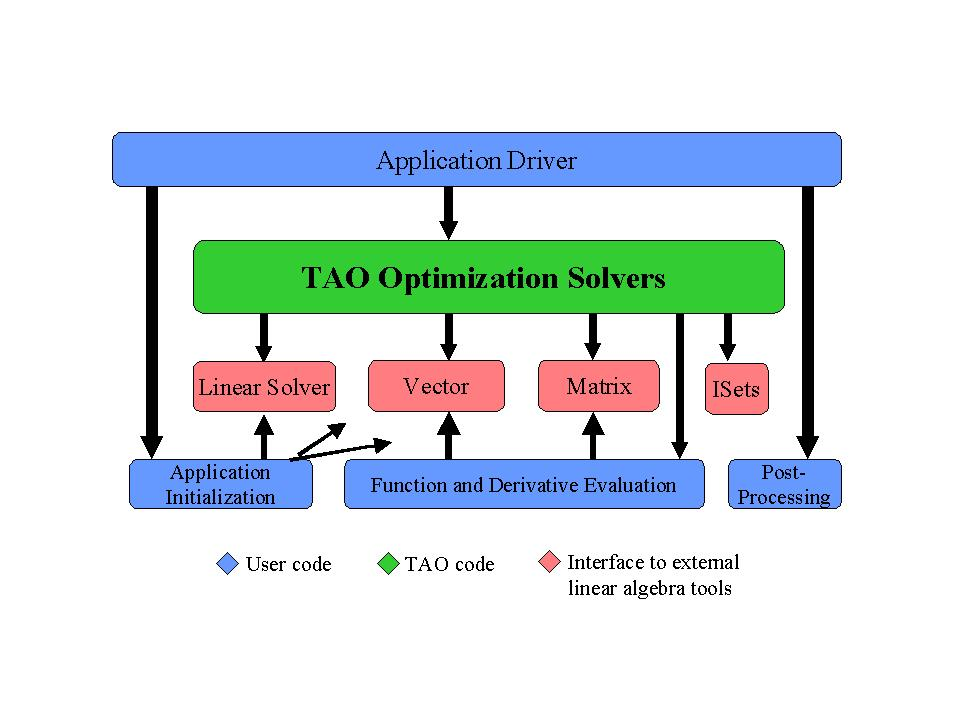
\includegraphics[height=2.5in]{../images/tao_pic3}}
\vfill
\end{slide}




\begin{slide}

\heading{Objective Function and Gradient Evaluation}

\begin{alltt}
\scriptsize \setlength{\baselineskip}{8pt}
\textcolor{blue}{
  typedef struct \{}          /* Used in the minimum surface area problem */
    \textcolor{blue}{int         mx, my;}            /* discretization in x, y directions */
    \textcolor{blue}{int         bmx, bmy, bheight;}             /* The size of the plate */
    \textcolor{blue}{double      bheight;}                     /* The height of the plate */
    \textcolor{blue}{double     *bottom, *top, *left, *right;}         /* boundary values */
  \} \textcolor{blue}{AppCtx;}

  \textcolor{blue}{int FormFunction}(TAO_SOLVER, \textcolor{red}{Vec x}, double *fcn, \textcolor{blue}{void *userCtx})\{
     \textcolor{blue}{AppCtx *user = (AppCtx *)userCtx;}
     ...
  \}
  \textcolor{blue}{int FormGradient}(TAO_SOLVER tao, \textcolor{red}{Vec x, Vec g}, \textcolor{blue}{void *userCtx})\{
     \textcolor{blue}{AppCtx *user = (AppCtx *)userCtx;}
     ...
  \}
  \textcolor{blue}{int FormHessian}(TAO_SOLVER tao,  \textcolor{red}{Vec x, Mat *H, Mat *H, int *flag}, \textcolor{blue}{void *userCtx})\{
     \textcolor{blue}{AppCtx *user = (AppCtx *)userCtx;}
     ...
  \}

\end{alltt}

\vfill

\end{slide}




\begin{slide}
\heading{Using TAO with PETSc}
\begin{alltt}
\scriptsize \setlength{\baselineskip}{8pt}
  TAO_SOLVER      tao;              /* TAO Optimization solver          */
  TAO_APPLICATION app;              /* TAO Application using PETSc      */
  \textcolor{blue}{AppCtx          user;             /* user-defined application context */}
  \textcolor{red}{Vec             x, g;             /* solution and gradient vectors    */
  Mat             H;                /* Hessian Matrix                   */}

  \textcolor{red}{VecCreateSeq(PETSC_COMM_SELF,n,&x);
  VecDuplicate(x,&g);
  MatCreateSeqAIJ(PETSC_COMM_SELF,n,n,nz,NULL,&H);}
  TaoCreate(PETSC_COMM_SELF,TAOLMVM,&tao);
  TaoPetscApplicationCreate(PETSC_COMM_SELF,&app);
  TaoSetPetscFunction(app,\textcolor{red}{x},\textcolor{blue}{FormFunction,(void *)&user});
  TaoSetPetscGradient(app,\textcolor{red}{g},\textcolor{blue}{FormGradient,(void *)&user});
  TaoSetPetscHessian(app,\textcolor{red}{H},\textcolor{red}{H},\textcolor{blue}{FormHessian,(void *)&user});
  TaoSetApplication(tao,app);
  TaoSolve(tao);
  \textcolor{red}{VecView(x,PETSC_VIEWER_STDOUT_SELF);}
\end{alltt}

\vfill

\end{slide}


\begin{slide}

\heading{Creating and Using a TAO Application}

\begin{alltt}
\scriptsize \setlength{\baselineskip}{8pt}
  TAO_SOLVER      tao;              /* TAO Optimization solver          */
  \textcolor{green}{TAO_APPLICATION app;              /* TAO Application using PETSc      */}
  AppCtx          user;             /* user-defined application context */
  Vec             x, g;             /* solution and gradient vectors    */
  Mat             H;                /* Hessian Matrix                   */

  VecCreateSeq(PETSC_COMM_SELF,n,&x);
  VecDuplicate(x,&g);
  MatCreateSeqAIJ(PETSC_COMM_SELF,n,n,nz,NULL,&H);
  TaoCreate(PETSC_COMM_SELF,TAOLMVM,&tao);
  \textcolor{green}{TaoPetscApplicationCreate(PETSC_COMM_SELF},\textcolor{green}{&app});
  \textcolor{green}{TaoSetPetscFunction}(\textcolor{green}{app},x,FormFunction,(void *)&user);
  \textcolor{green}{TaoSetPetscGradient}(\textcolor{green}{app},g,FormGradient,(void *)&user);
  \textcolor{green}{TaoSetPetscHessian}(\textcolor{green}{app},H,H,FormHessian,(void *)&user);
  TaoSetApplication(tao,app);
  TaoSolve(tao);
  VecView(x,PETSC_VIEWER_STDOUT_SELF);
\end{alltt}

\vfill

\end{slide}


\begin{slide}

\heading{Creating and Using a TAO Solver}

\begin{alltt}
\scriptsize \setlength{\baselineskip}{8pt}
  \textcolor{green}{TAO_SOLVER      tao;              /* TAO Optimization solver          */
  TAO_APPLICATION app;              /* TAO Application using PETSc      */}
  AppCtx          user;             /* user-defined application context */
  Vec             x, g;             /* solution and gradient vectors    */
  Mat             H;                /* Hessian Matrix                   */

  VecCreateSeq(PETSC_COMM_SELF,n,&x);
  VecDuplicate(x,&g);
  MatCreateSeqAIJ(PETSC_COMM_SELF,n,n,nz,NULL,&H);
  \textcolor{green}{TaoCreate(PETSC_COMM_SELF,}\textcolor{green}{TAOLMVM},\textcolor{green}{&tao});
  TaoPetscApplicationCreate(PETSC_COMM_SELF,&app);
  TaoSetPetscFunction(app,x,FormFunction,(void *)&user);
  TaoSetPetscGradient(app,g,FormGradient,(void *)&user);
  TaoSetPetscHessian(app,H,H,FormHessian,(void *)&user);
  \textcolor{green}{TaoSetApplication}(\textcolor{green}{tao, app});
  \textcolor{green}{TaoSolve}(\textcolor{green}{tao});
  VecView(x,PETSC_VIEWER_STDOUT_SELF);
\end{alltt}

\vfill

\end{slide}



\begin{slide}
\heading{A TAO Program Outline}
\begin{alltt}
\scriptsize \setlength{\baselineskip}{8pt}
  \textcolor{green}{TAO_SOLVER      tao;              /* TAO Optimization solver          */
  TAO_APPLICATION app;              /* TAO Application using PETSc      */}
  \textcolor{blue}{AppCtx          user;             /* user-defined application context */}
  \textcolor{red}{Vec             x, g;             /* solution and gradient vectors    */
  Mat             H;                /* Hessian Matrix                   */}

  \textcolor{red}{VecCreateSeq(PETSC_COMM_SELF,n,&x);
  VecDuplicate(x,&g);
  MatCreateSeqAIJ(PETSC_COMM_SELF,n,n,nz,NULL,&H);}
  \textcolor{green}{TaoCreate(}\textcolor{green}{PETSC_COMM_SELF},\textcolor{green}{TAOLMVM,&tao);}
  \textcolor{green}{TaoPetscApplicationCreate(}\textcolor{green}{PETSC_COMM_SELF},\textcolor{green}{&app);
  TaoSetPetscFunction(app},\textcolor{red}{x},\textcolor{blue}{FormFunction},\textcolor{blue}{(void *)&user});
  \textcolor{green}{TaoSetPetscGradient(app},\textcolor{red}{g},\textcolor{blue}{FormGradient},\textcolor{blue}{(void *)&user});
  \textcolor{green}{TaoSetPetscHessian(app},\textcolor{red}{H},\textcolor{red}{H},\textcolor{blue}{FormHessian},\textcolor{blue}{(void *)&user});
  \textcolor{green}{TaoSetApplication(tao,app);
  TaoSolve(tao);}
  \textcolor{red}{VecView(x,PETSC_VIEWER_STDOUT_SELF);}
\end{alltt}
\vfill
\end{slide}


\begin{slide}
\heading{Using PETSc Objects on Multiple Processors}

\begin{alltt}
\scriptsize \setlength{\baselineskip}{8pt}
  TAO_SOLVER      tao;              /* TAO Optimization solver          */
  TAO_APPLICATION app;              /* TAO Application using PETSc      */
  AppCtx          user;             /* user-defined application context */
  \textcolor{red}{Vec             x, g;             /* solution and gradient vectors    */
  Mat             H;                /* Hessian Matrix                   */

  VecCreateMPI(PETSC_COMM_WORLD,n,&x);}
  VecDuplicate(x,&g);
  \textcolor{red}{MatCreateMPIAIJ(PETSC_COMM_WORLD,nlocal,nlocal,n,n,d_nz,d_nnz,o_nz,o_nnz,&H);}
  TaoCreate(\textcolor{red}{PETSC_COMM_WORLD},TAOLMVM,&tao);
  TaoPetscApplicationCreate(\textcolor{red}{PETSC_COMM_WORLD},&app);
  TaoSetPetscFunction(app,x,\textcolor{blue}{FormFunction,(void *)&user});
  TaoSetPetscGradient(app,g,\textcolor{blue}{FormGradient,(void *)&user});
  TaoSetPetscHessian(app,H,H,\textcolor{blue}{FormHessian,(void *)&user});
  TaoSetApplication(tao,app);
  TaoSolve(tao);
  VecView(x,\textcolor{red}{PETSC_VIEWER_STDOUT_WORLD});
\end{alltt}

\vfill

\end{slide}


\begin{slide}

\heading{Convergence}

Absolute tolerances specify acceptable errors in the optimality of the function
and the constraints.
\[ f(x) \leq f(x^*) + \epsilon_{fatol} \]
Relative tolerances specify the number of significant digits required
in the solution and the constraints.
\[ 
f(x) \leq f(x^*) + \epsilon_{frtol} | f(x^*) |
\]

These tolerance can be changed
\begin{alltt}
\scriptsize \setlength{\baselineskip}{10pt}
    \textcolor{green}{int TaoSetTolerances(TAO_SOLVER solver,double fatol,double frtol,
                                           double catol,double crtol)}
\end{alltt}

\vfill

\end{slide}


\begin{slide}

\heading{TAO Basic Facilities}

\begin{list}{\reddiamond}{}
\item
TaoSetInitialSolution
\item
TaoSetVariableBounds
\item
TaoGetLinearSolver
\item 
TaoSetFromOptions
\item
TaoSetMonitor
\item
TaoView
\item
\ldots
\end{list}

\vfill

\end{slide}

\begin{slide}
\heading{Where Can We Find TAO?}

At {\bf http://www.mcs.anl.gov/tao}

\begin{list}{\reddiamond}{\leftmargin=1in}
\item
Source Code
\item
Documentation
\item
Installation Instructions
\item
Example Problems
\item
Additional Tutorials
\item
Performance Results
\item
Supported Architectures
\end{list}

\vfill

\end{slide}


\end{document}


\begin{slide}

\heading{}

\begin{list}{\reddiamond}{}
\item

\end{list}

\vfill

\end{slide}
